\section{Benchmark Results for the Onset of Rising Tone Chorus}
\label{sec:code}
We proceed with a series of simulations, employing our method to investigate the onset of the whistler-mode chorus
 in the  magnetosphere. The instability of the whistler wave typically arises from the electron temperature anisotropy  \cite{kennel1966a,kennel1966b} and the growth rate can be derived from the linear resonance condition.
 % near $\Omega \approx 0$.
In our simulation, the energetic electron distribution is bi-Maxwellian at the magnetic equator, 
%Moving away from the magnetic equator, the equilibrium distribution maintains the similar form as it does in the phase space by conventional coordinates $(s_i, p_\|, \phi, \varphi)$. The distribution function in new canonical variables is given directly by the canonical transformation in ref \cite{zheng2023a}, and we have 
\begin{equation}
    \begin{aligned}
        & f_{0}(\Omega, \mathcal{J}) =\frac{\omega_{c e 0}}{(2 \pi)^{3 / 2} v_{ \perp 0}^2 v_{ \| 0}} \cdot \exp \left(-\frac{k_l^2(\Omega+\Pi_i)^2}{2 v_{ \| 0}^2}\right) \\
        &\cdot\exp \left(-\frac{(\mathcal{J}+\Omega+\Pi_i) \omega_{c e 0}}{v_{ \perp 0}^2}\right)~,
        \end{aligned}
\end{equation}
where $v_{ \| 0}$
and $v_{ \perp 0}$ are the
%$\beta$ is the depth of the loss cone 
parallel and perpendicular thermal velocity of energetic electrons,
and 
the subscript $0$ denotes the magnetic equator.
%As a realistic model for, The Earth's magnetic field can be approximated as a dipole field and 
%the major component of 
The background magnetic field strength near the equator is approximated %represented
 by a parabolic function \cite{tao2014a}
\begin{equation}
    B(\lambda) = B_0 (1+ R_a \lambda ^2)~,
\end{equation}
where $R_a$ is the inhomogeneity parameter of the magnetic dipole field, $B_0$ is the magnetic field strength at the equator, and $\lambda$ is the magnetic latitude. %The distance  satisfies $s = L R_E \lambda$.
For the dipole field, 
%the magnetic strength decays as the cube of the radius increases, i.e.,
%\begin{equation}
 $   B_0 = B_{0g}/L^3$
%\end{equation}
where $B_{0g}\approx $0.3 G is the magnetic field of the Earth  at the equator 
%on the  surface of Earth 
and $L$ is the L-shell of the magnetic field line.
The background electron density along the magnetic field line  is  fit to a power law \cite{denton2004},
\begin{equation}
    n(\lambda) = n_0 (1+R_b \lambda^2)~,
\end{equation}
where $R_b$ represents the 
background cold plasma density inhomogeneity.
For the normalization in the simulation, 
 we use electron mass $m_e$, electron charge $e$, speed of light $c$ and background electron plasma frequency at the magnetic equator $\omega_{pe0}$ to normalize mass, charge, velocity and frequency.
Then the  units for the other quantities can be derived. 
For example,
the length $s $ is normalized to $ c/\omega_{pe0}$
and 
 the vector potential $A$ to $m_e c^2/e$.




   \begin{figure}[htbp]
        \centering
        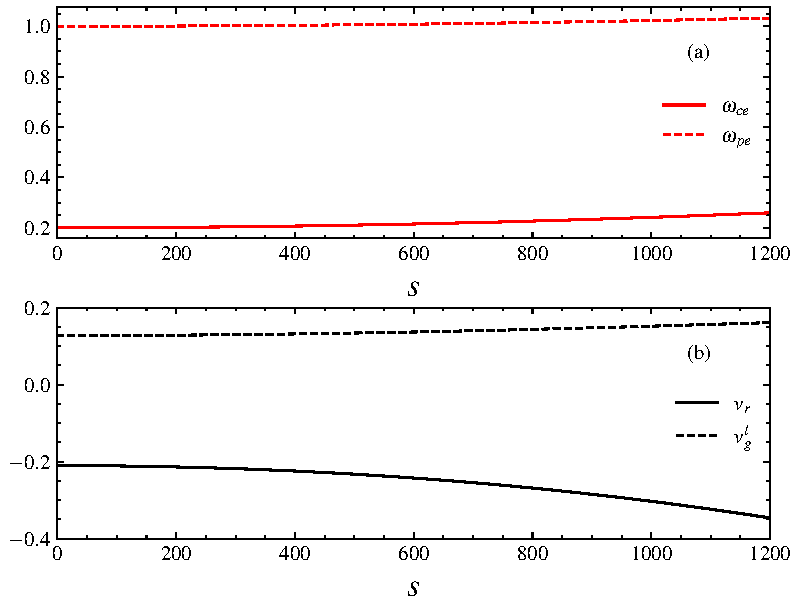
\includegraphics[scale=0.5]{cpc_img/fig_profile.pdf}
        \caption{(a) Background magnetic field and density profile. (b) Resonant and linear group velocity profile along the magnetic field line.}
        \label{fig.profile}
    \end{figure}
\subsection{Simulation configuration}

\begin{table}\label{tab.parameters}
    \centering
    \caption{Magnetic field and plasma parameters used in the simulation.\newline}
    \begin{tabular}{lc}
    \hline
     L-shell of the magnetic field line  & 5 \\
     Magnetic field inhomogeneity  $R_a$ &  4.5 \\
     Background cold plasma density inhomogeneity  $R_b$ &  1.0 \\
     Background electron gyrofrequency and plasma frequency at the equator & \makecell{ $\omega_{ce0} = 43929.6~\mathrm{rad/s}$\\$\omega_{pe0} = 5 \omega_{ce0}$  }\\
     Ratio of energetic to cold  electron density at the  equator &  $n_{h0} = 0.002$ \\ 
     Parallel and perpendicular thermal velocity of energetic electrons & \makecell{$v_{\perp 0} = 0.3 c$\\ $v_{\|0} = 0.15c$}  \\
    %Depth of the loss cone $\beta$ & 0 \\
    Size of the simulation domain  & \makecell{$\lambda \in [-15^\circ, 15^\circ]$ \\ $s \in [-6115,6115] c/\omega_{pe0}$} \\
    \hline
    \end{tabular}\\
    \end{table}
%(useless) Note that, since we apply the electron plasma frequency $\omega_{pe0}$ at the equator for time normalization, the value always be 1 desites the L-shell value, which gyrofrequency is dynamcally changes.
 
In conventional PIC simulations, the inhomogeneity ratio $R_a$ is often increased by one or two order of magnitudes to reduce the simulation cost.
%In contrast,
%However, one of the advantages of 
% is that we can
Benefiting from the scale-separated HEL  scheme,
 the realistic parameters for the Earth's dipole field
can be used in our numerical simulation.
The basic parameters 
of our simulation 
are given in Table (\ref{tab.parameters})
and the profiles of the background parameter are shown in Fig. \ref{fig.profile}.
%Meanwhile, 
The most unstable wave frequency $\omega_l$ used in the simulation 
%for the %determination of initial reference frame
% According to the choosen parameter in Tab. (\ref{tab.parameters}) and the definition of
 is determined from the linear growth rate  $\gamma_l$ \cite{gary_1993},
\begin{equation}
\begin{aligned}
    \gamma_l(s) & =\frac{\sqrt{2 \pi} \omega_{ce} v_g n_{h0} \omega_{pe0}^2}{4 k_l^2 v_{ \| 0}} e^{-\frac{\left(\omega_l-\omega_{c e}\right)^2}{2 k_l^2 v_{ \| 0}}}
    \cdot \left( \frac{T_{\perp 0}}{T_{\| 0}} \frac{\omega_{c e 0}-\omega_l}{\omega_{c e 0}}-1\right)~,
    \end{aligned}
\end{equation}
where 
 $n_{h0}$ is the density ratio of the energetic electrons to the background cold plasma at the magnetic equator,
the wave number $k_l$ satisfies the linear whistler disperison relation
\begin{equation}
    \frac{c^2 k_l^2(s)}{\omega_l^2} = 1 + \frac{\omega_{pe}^2(s)}{\omega_l(\omega_{ce}(s)-\omega_l)},
\end{equation}
and $v_g$ is the linear whistler group velocity,
\begin{equation}
    v_g(s) = \frac{2k_l(s)c^2 }{2\omega_l + \omega_{pe}^2(s)\omega_{ce}(s)/(\omega_{ce}(s)-\omega_l)^2}~.
\end{equation}
The temperature is given by the thermal velocity shown in Tab. (\ref{tab.parameters}).
For the  parameters in Tab. (\ref{tab.parameters}), 
the most unstable 
growth rate is $\gamma_l \simeq 3.24\times 10^{-4}$
and the corresponding 
frequency is $\omega_l = 0.061$, as shown by a scan of the parameter given in Fig.~\ref{fig.para}.
For the typical runs, we set the number of grids for wave solver to be 1001
which is equal to  the number of sampling points in $s$.
In the $\mathcal{J}$ dimension, we employ a delta function with only a single sampling point for $\mathcal{J}$. In the case of a non-delta distribution, tens of sampling points prove to be sufficient for $\mathcal{J}$ sampling.
For the $\xi,\Omega$ domain, the Eulerian grids are $31 \times 401$ for $\xi \in [0,2\pi]$ and $\Omega \in [-0.1,0.1]$.
\begin{figure}[htbp]
    \centering
    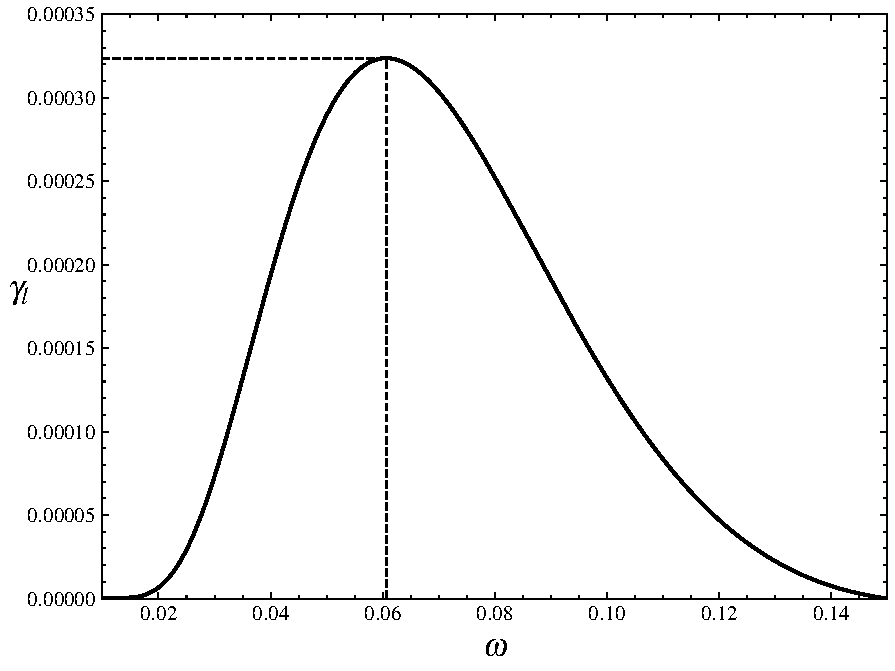
\includegraphics[scale=0.5]{cpc_img/fig_gamma1d.pdf}
    \caption{Linear growth rate $\gamma_l$ with respect to $\omega_l$ for the simulation parameters. The initial frequency of the wave is obtained from the most unstable frequency indicated by the vertical black line.}
    \label{fig.para}
\end{figure}

\subsection{Benchmarks results}
The linear physics are quantitatively verified in Fig. \ref{fig.linear}, where we calculate the growth rate and the velocity of the maximum wave amplitude location before nonlinear effects become dominant.
 %In the case of the  wave packet, we determine
  The trajectory of the propagating wave packet is determined theoretically using the integral of the linear group velocity,
\begin{equation}
    s(t) = s(0) + \int_0^{t} v_g(s(\tau)) \mathrm{d} \tau~.
\end{equation}
For the simulation,
 we track the movement of the maximum amplitude point. 
%Its propagation is in accord with the linear group velocity, 
 As shown in Fig. \ref{fig.linear}(a), 
 the wave peak indeed propagates at the linear group velocity during the linear stage.
 The 
 amplitude growth of the wave peak along its propagation path
%growth of the wave peak  along the propatation path 
is shown in Fig. \ref{fig.linear}(b)
and 
%Moreover, we  
 the growth rate is estimated by \cite{nogi2022}
\begin{equation}\label{eq.gm_ver}
        \gamma = \frac{1}{t_1-t_0}\log\frac{|a(s_1,t_1)|}{|a(s_0,t_0)|}~,
\end{equation}
where $s_0$ and $s_1$ are the points along the propagation path.
The  growth rate calculated from Eq. (\ref{eq.gm_ver}) is $\gamma \simeq 3.21\times10^{-4}$, which agrees with the theoretical linear growth rate shown in Fig. \ref{fig.para}.
%The results show the correctness of our simulation at linear stage.
\begin{figure}[htbp]
    \centering
    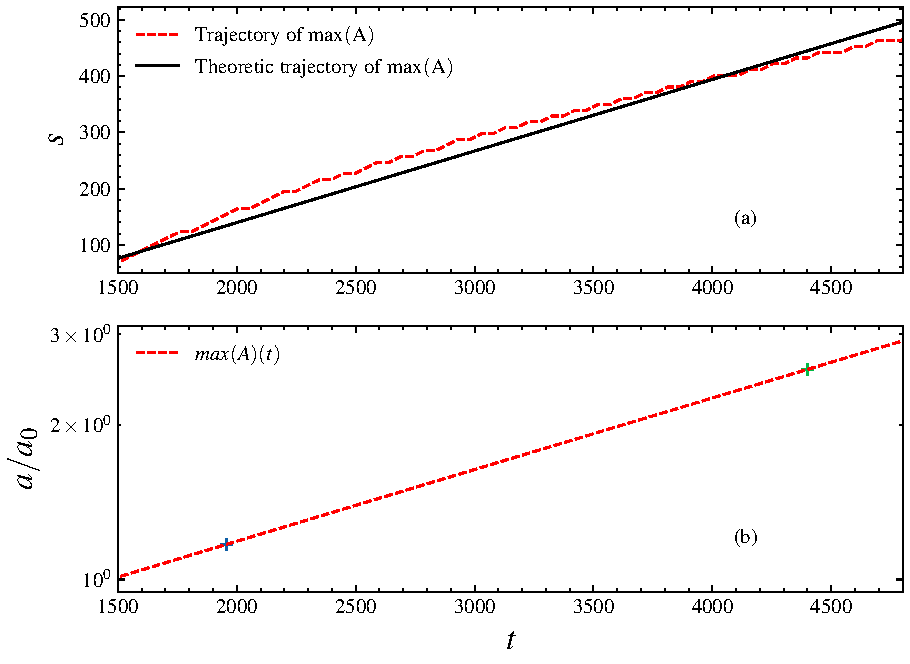
\includegraphics[scale=0.5]{cpc_img/fig_linear.pdf}
    \caption{ (a) Propagation trajectory of the linear wave packet with the maximum amplitude from the simulation (dashed line) and theory (solid line).  (b)  Growth of the wave peak amplitude with time along wave propagation path. The green crosses are the points used to caluclate the growth rate.}
    \label{fig.linear}
\end{figure}

In the nonlinear stage, the distribution of trapped electrons forms a  hole structure in $\xi-\Omega$ phase space. This phase space hole contributes to the nonlinear current, which in turn triggers the nonlinear frequency-chirping chorus wave. 
% The Hamiltonian for the resonant electrons has the form %\cite{}
% \begin{equation}
% H = \frac{k^2\Omega^2}{2} + \frac{\omega_b^2}{k^2}\left(\cos \xi + \alpha \xi \right)~,
% \end{equation}
The trapped electron experiences  an osillatory force from the wave and a noninertial force from background inhomogeneity. The forces can be described by a potential well with the form $\sin \xi + \alpha \xi$ with the parameter $\alpha$ as an inhomogeneity ratio \cite{omura2008,tao2020}.
% \begin{equation}\label{eq.alp}
%     \alpha \equiv \frac{1}{\omega_{b}^2}\left[\left(1 - 2\frac{v_r}{v_g}\right)\frac{\partial \omega}{\partial t}  -v_r^2 \frac{\partial k}{\partial s}+ \frac{\mathrm{\partial} \omega_{ce}}{\mathrm{\partial} s}\frac{k_i}{m_e}\mathcal{J}\right].
% \end{equation}
From 
the inflection point of the potential well,
%the potential well, 
we can find the X point of the phase space trajectory, 
\begin{equation}
    \xi_\mathrm{x} = - \arcsin \alpha,
\end{equation}
and the C point of the trajectory is obtained from the energy on the separatrix $e_\mathrm{spx} = \sin \xi_\mathrm{x} + \alpha \xi_\mathrm{x}$,
\begin{equation}
    \sin \xi_\mathrm{c} + \alpha \xi_\mathrm{c} = e_\mathrm{spx}.
\end{equation}
The shape of the hole, specifically its boundary, can be analytically described as follows \cite{omura2008}:
\begin{equation}\label{eq.Omega_b}
    \Omega(\xi) = \pm \frac{\omega_b}{k^2} \sqrt{2 (e_\mathrm{spx}-\cos \xi - \alpha \xi)}~,
\end{equation}
where $k$ is the wave number and $\omega_b$
%\equiv \sqrt{k^2 v_\perp a}$ 
is the trapped particle bounce frequency.
Using
the simulation data we obtain the values of $k \simeq 0.649$, $\omega_b \simeq 0.007$, and $\alpha \simeq 0.08$ at a specific location $s\simeq 2107$. Then the boundary of the hole can be obtained using Eq. (\ref{eq.Omega_b}).
As shown 
in Fig.~\ref{fig.hole},
the shape of the hole in the nonlinear simulation
closely matches  the theoretical predictions.
%we present a typical electron phase-space hole observed at a specific location $s$ in the late nonlinear stage. We determine the corresponding values of $k \simeq 0.649$, $\omega_b \simeq 0.007$, $\alpha \simeq 0.08$ based on the simulation data at that location. Additionally, we illustrated the boundary of the hole using the equation (\ref{eq.Omega_b}). Notably, the shape of the hole closely aligns with the theoretical predictions.

\begin{figure}[htbp]
    \centering
    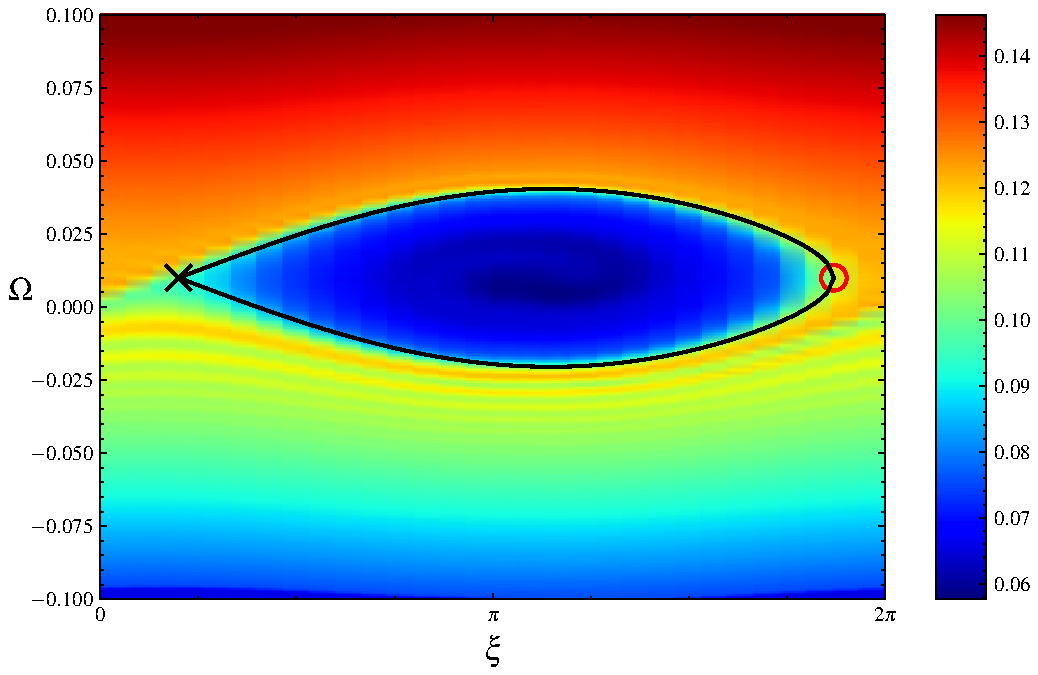
\includegraphics[scale=0.5]{cpc_img/fig_hole.pdf}
    \caption{Phase-space hole  formed by trapped electrons at $s\simeq 2107$ in the wave field. The X, C points on the left and right ends and the boundary of the hole (black solid line) are obtained from theory.}
    \label{fig.hole}
\end{figure}


